\documentclass{report}
\usepackage[a4paper,total={7in,10in}]{geometry}

\usepackage{amsmath}
\usepackage{amssymb}
\usepackage{enumitem}
\usepackage{tikz, pgfplots}
\usepackage{multicol}
\usepackage{setspace}
\usepackage{graphicx}
\usetikzlibrary{arrows}

\setcounter{chapter}{10}
\setcounter{section}{2}

\newcommand{\sol}{\vspace{1em}\\\textbf{Sol.}}
\newcommand{\proof}{\vspace{1em}\\\textbf{Proof.}}
\newcommand{\eos}{ \qquad \square}
\counterwithout{equation}{chapter} % remove the chapter number
\newcommand\numberthis{\addtocounter{equation}{1}\tag{\theequation}}

\begin{document}
\section*{Revision Exercise 5}

\onehalfspacing
\begin{enumerate}
    \item Conic curve equations are given as follows. Identify the type of curve and find
          their eccentricity $e$:
          \begin{enumerate}
              \item $2x^2-y^2+6x+2y+3=0$
                    \sol{}
                    \begin{align*}
                        2x^2+6x-y^2+2y                                & = -3                                 \\
                        2(x^2+3x) - (y^2-2y)                          & = -3                                 \\
                        2\left(x^2+3x+\frac{9}{4}\right) - (y^2-2y+1) & = -3 + 2\left(\frac{9}{4}\right) - 1 \\
                        2\left(x+\frac{3}{2}\right)^2 - (y-1)^2       & = \dfrac{1}{2}                       \\
                        4\left(x+\frac{3}{2}\right)^2 - 2(y-1)^2      & = 1
                    \end{align*}
                    The equation is of the form
                    \begin{equation*}
                        \frac{(x-h)^2}{a^2} - \frac{(y-k)^2}{b^2} = 1
                    \end{equation*}
                    Therefore, the curve is a \textbf{hyperbola} with $a^2=\dfrac{1}{4}$ and $b^2=\dfrac{1}{2}$.

                    The eccentricity of the hyperbola is given by
                    \begin{align*}
                        e & = \dfrac{1}{\dfrac{1}{2}}\sqrt{\dfrac{1}{4} + \dfrac{1}{2}} \\
                          & = 2\sqrt{\dfrac{3}{4}}                                      \\
                          & = \sqrt{3} \eos
                    \end{align*}

              \item $y^2-4y-4x+16=0$
                    \sol{}
                    \begin{align*}
                        y^2-4y-4x+16     & = 0       \\
                        y^2-4y+16        & = 4x      \\
                        (y-2)^2 - 4 + 16 & = 4x      \\
                        (y-2)^2          & = 4x - 12 \\
                        (y-2)^2          & = 4(x-3)
                    \end{align*}
                    The equation is of the form
                    \begin{equation*}
                        (y-k)^2 = 4a(x-h)
                    \end{equation*}
                    Therefore, the curve is a \textbf{parabola}.

                    The eccentricity of the parabola is $1$. $\eos$

                    \newpage
              \item $x^2+4y^2+8x-16y-17=0$
                    \sol{}
                    \begin{align*}
                        x^2+8x+4y^2-16y-17                        & = 0  \\
                        (x^2+8x+16) - 16 + 4(y^2-4y + 4) - 16 -17 & = 0  \\
                        (x+4)^2 + 4(y-2)^2                        & = 49 \\
                        \frac{(x+4)^2}{49} + \frac{4(y-2)^2}{49}  & = 1
                    \end{align*}
                    The equation is of the form
                    \begin{equation*}
                        \frac{(x-h)^2}{a^2} + \frac{(y-k)^2}{b^2} = 1
                    \end{equation*}
                    Therefore, the curve is an \textbf{ellipse} with $a^2=49$ and $b^2=\dfrac{49}{4}$.

                    The eccentricity of the ellipse is given by
                    \begin{align*}
                        e & = \dfrac{1}{7}\sqrt{49 - \dfrac{49}{4}}  \\
                          & = \dfrac{1}{7}\sqrt{\dfrac{147}{4}}      \\
                          & = \dfrac{1}{7}\cdot\dfrac{\sqrt{147}}{2} \\
                          & = \dfrac{\sqrt{3}}{2} \eos
                    \end{align*}

              \item $x^2-y^2-4x+2y-1=0$
                    \sol{}
                    \begin{align*}
                        x^2-4x-y^2+2y-1                 & = 0 \\
                        x^2-4x-y^2+2y                   & = 1 \\
                        (x^2-4x+4) - 4 - (y^2-2y+1) - 1 & = 1 \\
                        (x-2)^2 - (y-1)^2               & = 6 \\
                    \end{align*}
                    The equation is of the form
                    \begin{equation*}
                        (x-h)^2 - (y-k)^2 = a^2
                    \end{equation*}
                    Therefore, the curve is a \textbf{rectangular hyperbola} with $a^2=6$.

                    The eccentricity of any rectangular hyperbola $\sqrt{2}$. $\eos$
          \end{enumerate}

          \newpage

    \item Discuss the conic curve represented by $kx^2+2y^2-8x=0$ for the three cases of
          $k>0$, $k=0$, and $k<0$. \sol{}

          When $k>0$,
          \begin{align*}
              kx^2+2y^2-8x                                                                                               & = 0             \\
              kx^2 - 8x + 2y^2                                                                                           & = 0             \\
              k\left(x^2 - \dfrac{8}{k}x\right) + 2y^2                                                                   & = 0             \\
              k\left(x^2 - 2\cdot\dfrac{4}{k}x + \left(\dfrac{4}{k}\right)^2 - \left(\dfrac{4}{k}\right)^2\right) + 2y^2 & = 0             \\
              k\left(x^2 - 2\cdot\dfrac{4}{k}x + \left(\dfrac{4}{k}\right)^2\right) - \dfrac{16}{k} + 2y^2               & = 0             \\
              k\left(x - \dfrac{4}{k}\right)^2 + 2y^2                                                                    & = \dfrac{16}{k} \\
              \dfrac{k\left(x - \dfrac{4}{k}\right)^2}{\dfrac{16}{k}} + \dfrac{2y^2}{\dfrac{16}{k}}                      & = 1             \\
              \dfrac{k^2\left(x - \dfrac{4}{k}\right)^2}{16} + \dfrac{ky^2}{8}                                           & = 1
          \end{align*}
          The equation is of the form
          \begin{equation*}
              \frac{(x-h)^2}{a^2} + \frac{(y-k)^2}{b^2} = 1
          \end{equation*}
          Therefore, the curve is an \textbf{ellipse}. $\eos$

          When $k=0$,
          \begin{align*}
              0x^2+2y^2-8x & = 0  \\
              2y^2-8x      & = 0  \\
              2y^2         & = 8x \\
              y^2          & = 4x
          \end{align*}
          The equation is of the form
          \begin{equation*}
              y^2 = 4ax
          \end{equation*}
          Therefore, the curve is a \textbf{parabola}. $\eos$

          When $k<0$,
          \begin{align*}
              -kx^2+2y^2-8x                                                    & = 0 \\
              \dfrac{k^2\left(x + \dfrac{4}{k}\right)^2}{16} - \dfrac{ky^2}{8} & = 1
          \end{align*}
          The equation is of the form
          \begin{equation*}
              \frac{(x-h)^2}{a^2} - \frac{(y-k)^2}{b^2} = 1
          \end{equation*}
          Therefore, the curve is a \textbf{hyperbola}. $\eos$

          \newpage
    \item Find the equations of curves that satisfy the following conditions:
          \begin{enumerate}
              \item An ellipse with center at $O'(-2,1)$, semi-major axis length 10, foci on lines
                    parallel to the $x$-axis, and the distance between the two foci is 12. \sol{}

                    Move the center of the ellipse to the origin by translating the axes such that
                    \begin{align*}
                        x' & = x + 2 \qquad \text{and} \qquad y' = y - 1
                    \end{align*}
                    Since the foci are on lines parallel to the $x$-axis, the equation of the ellipse is
                    \begin{align*}
                        \frac{(x')^2}{a^2} + \frac{(y')^2}{b^2} & = 1        \\
                        a                                       & = 10       \\
                        2ae                                     & = 12       \\
                        ae                                      & = 6        \\
                        b^2                                     & = 100 - 36 \\
                                                                & = 64
                    \end{align*}
                    Therefore, the equation of the ellipse is
                    \begin{align*}
                        \frac{(x')^2}{100} + \frac{(y')^2}{64}   & = 1      \\
                        \frac{(x+2)^2}{100} + \frac{(y-1)^2}{64} & = 1 \eos
                    \end{align*}
              \item A hyperbola with imaginary axis length of 8, vertices at $\mathrm{A}(2,1)$ and
                    $\mathrm{A}'(2,-5)$. \sol{}

                    The center of the hyperbola is at the midpoint of the vertices, which is at
                    $\left(2,\dfrac{1+(-5)}{2}\right) = \left(2,-2\right)$.

                    Move the center of the hyperbola to the origin by translating the axes such
                    that
                    \begin{align*}
                        x' & = x - 2 \qquad \text{and} \qquad y' = y + 2
                    \end{align*}
                    The vertices of the hyperbola are now at $(0, 3)$ and $(0, -3)$.

                    Since the vertices are on the $y$-axis, the equation of the hyperbola is of the
                    form
                    \begin{equation*}
                        \frac{(y')^2}{a^2} - \frac{(x')^2}{b^2} = 1
                    \end{equation*}
                    The imaginary axis length is $2b=8$, so $b=4$.

                    The vertices are at $(0, \pm 3)$, so $a=3$. Therefore, the equation of the
                    hyperbola is
                    \begin{align*}
                        \frac{(y+2)^2}{9} - \frac{(x-2)^2}{16} & = 1 \eos
                    \end{align*}

                    \newpage
              \item Foci at $\mathrm{F}(3,-3)$, directrix equation is $\mathrm{y}=1$ for a
                    parabola. \sol{}

                    Let any point on the parabola be $\mathrm{P}(x,y)$.
                    \begin{align*}
                        (x-3)^2 + (y+3)^2           & = \left(\dfrac{y-1}{1}\right)^2 \\
                        (x-3)^2 + (y+3)^2           & = (y-1)^2                       \\
                        x^2 - 6x + 9 + y^2 + 6y + 9 & = y^2 - 2y + 1                  \\
                        x^2 - 6x + 17 + 8y          & = 0                             \\
                        (x - 3)^2 + 8 + 8y          & = 0                             \\
                        (x - 3)^2                   & = -8y - 8                       \\
                        (x - 3)^2                   & = -8(y + 1) \eos
                    \end{align*}
          \end{enumerate}

    \item Lazy to do. =)

    \item A straight line passing through the focus of the parabola $y^2=4ax$ intersects
          the parabola at two points with vertical coordinates $y_1$ and $y_2$. Prove
          that $y_1 \cdot y_2 = -4a^2$. \proof{}

          The focus of the parabola is at $(a, 0)$.

          Let the two points of intersection be $\mathrm{A}(x_1, y_1)$ and
          $\mathrm{B}(x_2, y_2)$.

          Substituting $(x_1, y_1)$ and $(x_2, y_2)$ into the equation of the parabola,
          we get
          \begin{align*}
              y_1^2                                  & = 4ax_1                                                    \\
              x_1                                    & = \dfrac{y_1^2}{4a}                                        \\
              y_2^2                                  & = 4ax_2                                                    \\
              x_2                                    & = \dfrac{y_2^2}{4a}                                        \\
              \dfrac{0 - y_1}{a - x_1}               & = \dfrac{y_2 - y_1}{x_2 - x_1}                             \\
              \dfrac{-y_1}{a - \dfrac{y_1^2}{4a}}    & = \dfrac{y_2 - y_1}{\dfrac{y_2^2}{4a} - \dfrac{y_1^2}{4a}} \\
              \dfrac{-y_1}{\dfrac{4a^2 - y_1^2}{4a}} & = \dfrac{y_2 - y_1}{\dfrac{y_2^2 - y_1^2}{4a}}             \\
              \dfrac{-y_1}{4a^2 - y_1^2}             & = \dfrac{y_2 - y_1}{y_2^2 - y_1^2}                         \\
              \dfrac{-y_1}{4a^2 - y_1^2}             & = \dfrac{y_2 - y_1}{(y_2 - y_1)(y_2 + y_1)}                \\
              \dfrac{-y_1}{4a^2 - y_1^2}             & = \dfrac{1}{y_2 + y_1}                                     \\
              -y_1(y_2 + y_1)                        & = 4a^2 - y_1^2                                             \\
              -y_1y_2 - y_1^2                        & = 4a^2 - y_1^2                                             \\
              -y_1y_2                                & = 4a^2                                                     \\
              y_1y_2                                 & = -4a^2 \eos
          \end{align*}

          \newpage
    \item In the figure, there is a parabolic arch bridge. When the water surface is at
          $l$, the height of the arch from the water surface is $2$ m, and the width of
          the water surface is $4$ m. After the water surface descends by $1$ m, what is
          the new width of the water surface?
          \begin{center}
              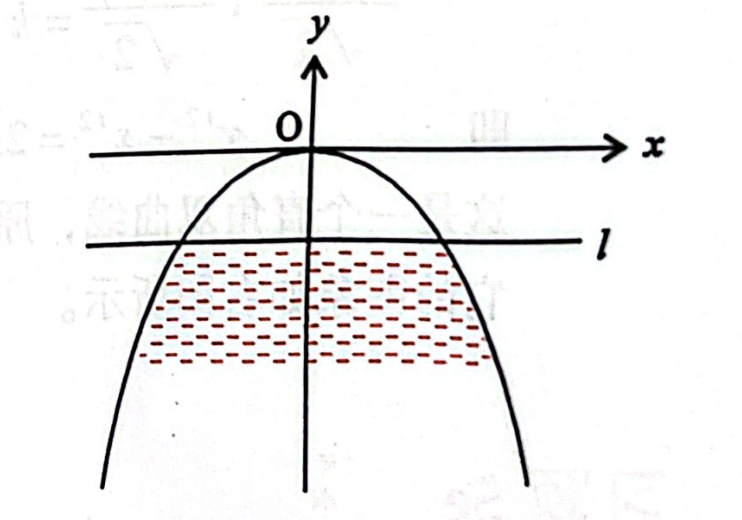
\includegraphics[scale=0.25]{./assets/reex56.png}
          \end{center}
          \ \sol{}

          Let the equation of the parabola be of the form
          \begin{equation*}
              x^2 = 4ay
          \end{equation*}
          When $x = 2$, $y = -2$
          \begin{align*}
              2^2 & = 4a(-2)        \\
              4   & = -8a           \\
              a   & = -\dfrac{1}{2}
          \end{align*}
          Therefore, the equation of the parabola is
          \begin{equation*}
              x^2 = -2y
          \end{equation*}
          When $y = -3$,
          \begin{align*}
              x^2 & = -2(-3)       \\
              x^2 & = 6            \\
              x   & = \pm \sqrt{6}
          \end{align*}
          Hence, the new width of the water surface is $2\sqrt{6} \approx 4.9$m. $\eos$

          \newpage
    \item The parabola $y^2=4x+4$ intersects the line $y=2x-2$. A chord $\mathrm{AB}$ is
          parallel to the $x$-axis, and the $y$-coordinate of points on the chord is $t$.
          Find the range of $t$ and the length of the chord $\mathrm{AB}$.
          \begin{center}
              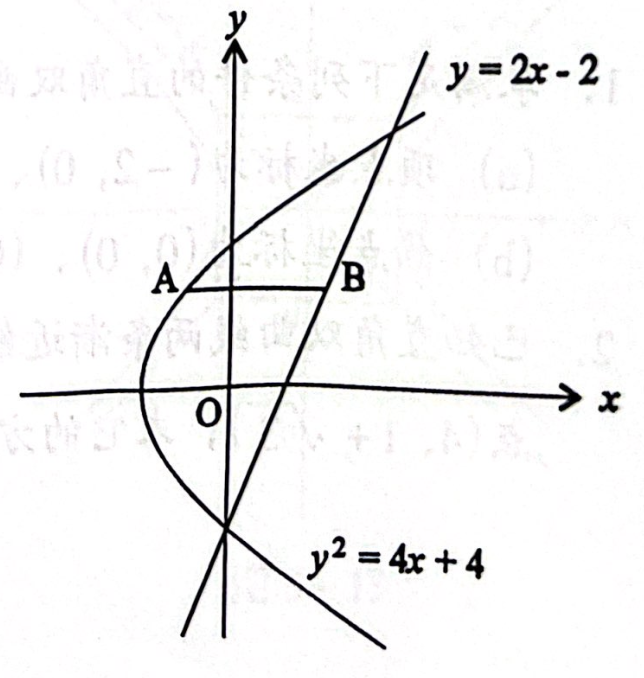
\includegraphics[scale=0.25]{./assets/reex57.png}
          \end{center}
          \ \sol{}

          Substituting $y=2x-2$ into the equation of the parabola, we get
          \begin{align*}
              (2x-2)^2  & = 4x+4                          \\
              4x^2-8x+4 & = 4x+4                          \\
              4x^2-12x  & = 0                             \\
              4x(x-3)   & = 0                             \\
              x         & = 0 \quad \text{or} \quad x = 3
          \end{align*}
          When $x=0$, $y=-2$, and when $x=3$, $y=4$. Therefore, the range of $t$ is $-2 \leq t \leq 4$. $\eos$

          When $y = t$,
          \begin{align*}
              A\left(\dfrac{t^2 - 4}{4}, t\right) \\
              B\left(\dfrac{t + 2}{2}, t\right)
          \end{align*}
          The length of the chord $\overline{AB}$ is
          \begin{align*}
              |\overline{AB}| & = \sqrt{\left(\dfrac{t + 2}{2} - \dfrac{t^2 - 4}{4}\right)^2 + (t - t)^2} \\
                              & = \sqrt{\left(\dfrac{2t + 4 - t^2 + 4}{4}\right)^2}                       \\
                              & = \sqrt{\left(\dfrac{-t^2 + 2t + 8}{4}\right)^2}                          \\
                              & = \dfrac{1}{4}(t + 2)(4 - t) \eos
          \end{align*}

          \newpage
    \item For a line segment $\overline{AB}$ with length 1, where the endpoints $A$ and
          $B$ move along the $x$-axis and $y$-axis respectively, let $P$ be a point on
          $\overline{AB}$ such that $|\overline{PA}|:|\overline{PB}|=m:n$. Find the
          equation of the locus of point $P$, and state what type of curve it is. \sol{}

          Since the length of $\overline{AB}$ is 1,
          \begin{align*}
              x^2 + y^2 & = 1
          \end{align*}
          Let the coordinates of $A$ and $B$ be $(x, 0)$ and $(0, y)$ respectively, and
          the coordinates of $P$ be $(s, t)$.
          \begin{align*}
              (s, t) & = \left(\dfrac{nx}{m+n}, \dfrac{my}{m+n}\right) \\
              s      & = \dfrac{nx}{m+n}                               \\
              x      & = \dfrac{(m+n)s}{n}                             \\
              t      & = \dfrac{my}{m+n}                               \\
              y      & = \dfrac{(m+n)t}{m}
          \end{align*}
          Substituting the equations of $x$ and $y$ into the equation of the circle, we get
          \begin{align*}
              \left(\dfrac{(m+n)s}{n}\right)^2 + \left(\dfrac{(m+n)t}{m}\right)^2 & = 1 \\
              \dfrac{(m+n)^2s^2}{n^2} + \dfrac{(m+n)^2t^2}{m^2}                   & = 1
          \end{align*}
          Hence, the equation of the locus of point $P$ is
          \begin{align*}
              \dfrac{(m+n)^2x^2}{n^2} + \dfrac{(m+n)^2y^2}{m^2} & = 1 \eos
          \end{align*}
          And the type of curve is an \textbf{ellipse}. $\eos$

          \newpage
    \item Find a point on the ellipse $\dfrac{x^2}{25} + \dfrac{y^2}{9} = 1$ such that
          the angle formed by the lines connecting it to the two foci of the ellipse is a
          right angle. \sol{}

          The foci of the ellipse are at $(\pm 4, 0)$.

          Let the point on the ellipse be $\mathrm{P}(x, y)$.
          \begin{align*}
              \dfrac{x^2}{25} + \dfrac{y^2}{9}                & = 1                                      \\
              9x^2 + 25y^2                                    & = 225                                    \\
              25y^2                                           & = 225 - 9x^2                             \\
              y^2                                             & = 9 - \dfrac{9}{25}x^2                   \\
              \\
              \dfrac{y - 0}{x - 4} \cdot \dfrac{y - 0}{x + 4} & = -1                                     \\
              \dfrac{y^2}{x^2 - 16}                           & = -1                                     \\
              y^2                                             & = -x^2 + 16                              \\
              9 - \dfrac{9}{25}x^2                            & = -x^2 + 16                              \\
              \dfrac{16}{25}x^2                               & = 7                                      \\
              x^2                                             & = \dfrac{175}{16}                        \\
              x                                               & = \pm \dfrac{5\sqrt{7}}{4}               \\
              y^2                                             & = 9 - \dfrac{9}{25}\times\dfrac{175}{16} \\
              y                                               & = \pm \dfrac{9}{4}
          \end{align*}
          Therefore, the points on the ellipse are $\left(\dfrac{5\sqrt{7}}{4}, \dfrac{9}{4}\right)$, $\left(\dfrac{5\sqrt{7}}{4}, -\dfrac{9}{4}\right)$, $\left(-\dfrac{5\sqrt{7}}{4}, \dfrac{9}{4}\right)$, and $\left(-\dfrac{5\sqrt{7}}{4}, -\dfrac{9}{4}\right).$ $\eos$

          \newpage
    \item Given that the vertex of a parabola lies at the center of the ellipse
          $\dfrac{x^2}{100} + \dfrac{y^2}{64} = 1$ and one focus lies on the right focus
          of the ellipse, find the intersection points of the ellipse and the parabola.
          \sol{}

          The center of the ellipse is at the origin, and the foci are at $(\pm 6, 0)$.

          Let the equation of the parabola be of the form
          \begin{equation*}
              y^2 = 4ax
          \end{equation*}
          The focus of the parabola is at $(6, 0)$, therefore $a=6$. The equation of the parabola is
          \begin{align*}
              y^2 & = 24x
          \end{align*}
          Substituting the equation of the parabola into the equation of the ellipse, we get
          \begin{align*}
              \frac{x^2}{100} + \frac{24x}{64}                               & = 1                             \\
              \frac{x^2}{100} + \frac{3x}{8}                                 & = 1                             \\
              8x^2 + 300x - 800                                              & = 0                             \\
              2x^2 + 75x - 200                                               & = 0                             \\
              (x + 40)(2x - 5)                                               & = 0                             \\
              x                               = -40 \text{ (rejected)} \quad & \text{or} \quad x = \frac{5}{2} \\
              y^2                                                            & = 24\left(\frac{5}{2}\right)    \\
              y^2                                                            & = 60                            \\
              y                                                              & = \pm 2\sqrt{15}
          \end{align*}
          Therefore, the intersection points of the ellipse and the parabola are at $\left(\dfrac{5}{2}, 2\sqrt{15}\right)$ and $\left(\dfrac{5}{2}, -2\sqrt{15}\right)$. $\eos$

    \item Find the equation of the hyperbola with eccentricity $e=\dfrac{5}{4}$ that
          shares a common focus with the ellipse $\dfrac{x^2}{49} + \dfrac{y^2}{24} = 1$.
          \sol{}

          The foci of the ellipse are at $(\pm 5, 0)$.

          Since the foci of the hyperbola are at $(\pm ae, 0)$, the equation of the
          hyperbola is of the form
          \begin{align*}
              \frac{x^2}{a^2} - \frac{y^2}{b^2} & = 1                            \\
              ae                                & = 5                            \\
              a                                 & = \dfrac{5}{\dfrac{5}{4}}  = 4 \\
              b^2                               & = a^2e^2 - a^2 = 25 - 16 = 9
          \end{align*}
          Therefore, the equation of the hyperbola is
          \begin{align*}
              \frac{x^2}{16} - \frac{y^2}{9} & = 1 \eos
          \end{align*}

    \item The cross-section of an oil tank on a tanker truck is an ellipse with a major
          axis length of $1.5 \, \text{m}$ and a minor axis length of $1 \, \text{m}$. If
          the length of the tank is $4 \, \text{m}$, find its volume. Given the formula
          for the area of an ellipse $S=\pi ab$ (where $a$ and $b$ are the lengths of the
          semi-major and semi-minor axes respectively), and assuming the density of
          gasoline is $0.7 \, \text{g/cm}^3$, find the maximum weight of gasoline the
          tank can hold in kilograms. \sol{}

          Let the equation of the cross section of the ellipse be
          \begin{equation*}
              \frac{x^2}{\left(0.75\right)^2} + \frac{y^2}{\left(0.5\right)^2} = 1
          \end{equation*}
          Hence, the volume of the tank is approximately
          \begin{align*}
              V & = \pi abh                                \\
                & = \pi \left(0.75\right)\left(0.5\right)4 \\
                & = 1.5\pi                                 \\
                & \approx 4.71 \, \text{m}^3 \eos
          \end{align*}
          The maximum weight of gasoline the tank can hold is approximately
          \begin{align*}
              W & = \text{density} \times \text{volume}          \\
                & = \dfrac{0.7}{1000} \times 4.71 \times 1000000 \\
                & = 3297 \, \text{kg} \eos
          \end{align*}

    \item Given the equations of two ellipses $\mathcal{C}_1: x^2 + 9y^2 - 45 = 0$ and
          $\mathcal{C}_2: x^2 + 9y^2 - 6x - 27 = 0$:
          \begin{enumerate}
              \item Find the coordinates of the centers and foci of these two ellipses. \sol{}

                    For $\mathcal{C}_1$:
                    \begin{align*}
                        x^2 + 9y^2 - 45                & = 0  \\
                        x^2 + 9y^2                     & = 45 \\
                        \frac{x^2}{45} + \frac{y^2}{5} & = 1
                    \end{align*}
                    The center of the ellipse is at the origin, and the foci are at $(\pm 2\sqrt{10}, 0)$ $\eos$

                    For $\mathcal{C}_2$:
                    \begin{align*}
                        x^2 + 9y^2 - 6x - 27                 & = 0  \\
                        x^2 - 6x + 9y^2 - 27                 & = 0  \\
                        (x - 3)^2 - 9 + 9y^2 - 27            & = 0  \\
                        (x - 3)^2 + 9y^2                     & = 36 \\
                        \frac{(x - 3)^2}{36} + \frac{y^2}{4} & = 1
                    \end{align*}
                    The center of the ellipse is at $(3, 0)$, and the foci are at $(3 \pm 4\sqrt{2}, 0)$ $\eos$

                    \newpage
              \item Find the equation of a circle passing through the intersection points of these
                    two ellipses and tangent to the line $x - 2y + 11 = 0$. \sol{}
                    \begin{align*}
                        x^2 + 9y^2 - 45          & = 0                     \\
                        9y^2                     & = 45 - x^2              \\
                        y^2                      & = 5 - \dfrac{1}{9}x^2   \\
                        x^2 + 9y^2 - 6x - 27     & = 0                     \\
                        x^2 + 45 - x^2 - 6x - 27 & = 0                     \\
                        6x                       & = 18                    \\
                        x                        & = 3                     \\
                        y^2                      & = 5 - \dfrac{1}{9}(3)^2 \\
                        y^2                      & = 4                     \\
                        y                        & = \pm 2
                    \end{align*}
                    The intersection points are at $(3, 2)$ and $(3, -2)$.

                    Let the equation of the circle be of the form
                    \begin{equation*}
                        (x - h)^2 + (y - k)^2 = r^2
                    \end{equation*}
                    Substituting the intersection points into the equation of the circle, we get
                    \begin{align*}
                        (3 - h)^2 + (2 - k)^2  & = r^2 \\
                        (3 - h)^2 + (-2 - k)^2 & = r^2
                    \end{align*}
                    Since the circle is tangent to the line $x - 2y + 11 = 0$, the distance from the center of the circle to the line is equal to the radius of the circle. Therefore,
                    \begin{align*}
                        \frac{|1(h) - 2(k) + 11|}{\sqrt{1^2 + 2^2}} & = r                         \\
                        |h - 2k + 11|                               & = \sqrt{5}r                 \\
                        5r^2                                        & = (h - 2k + 11)^2           \\
                        r^2                                         & = \frac{(h - 2k + 11)^2}{5}
                    \end{align*}
                    Substituting the value of $r^2$ into the equation of the circle, we get
                    \begin{align*}
                        (3 - h)^2 + (2 - k)^2  & = \frac{(h - 2k + 11)^2}{5} \\
                        (3 - h)^2 + (-2 - k)^2 & = \frac{(h - 2k + 11)^2}{5}
                    \end{align*}
                    Solving the two equations, we get $h = -1$, $k = 0$, or $h = 14$, $k = 0$.

                    \newpage
                    Substituting the values of $h$ and $k$ into $r^2 = \dfrac{(h - 2k + 11)^2}{5}$,
                    we get $r^2 = 20$ or $r^2 = 125$. Hence, the equation of the circle is
                    \begin{align*}
                        (x + 1)^2 + y^2     & = 20     \\
                        x^2 + 2x + 1 + y^2  & = 20     \\
                        x^2 + y^2 + 2x - 19 & = 0 \eos
                    \end{align*}
                    or
                    \begin{align*}
                        (x - 14)^2 + y^2      & = 125    \\
                        x^2 - 28x + 196 + y^2 & = 125    \\
                        x^2 + y^2 - 28x + 71  & = 0 \eos
                    \end{align*}
          \end{enumerate}

    \item If the eccentricity of a hyperbola is $2$, find the angle between its two
          asymptotes. \sol{}
          \begin{align*}
              e                                       & = \dfrac{c}{a}                               \\
              \dfrac{c^2}{a^2}                        & = 4                                          \\
              \dfrac{a^2 + b^2}{a^2}                  & = 4                                          \\
              1 + \dfrac{b^2}{a^2}                    & = 4                                          \\
              \dfrac{b^2}{a^2}                        & = 3                                          \\
              \dfrac{b}{a}                            & = \pm\sqrt{3}                                \\
              \tan\theta                              & = \pm\sqrt{3}                                \\
              \theta                 = 60^\circ \quad & \text{or} \quad 120^\circ (\text{ rejected})
          \end{align*}
          Hence, the angle between the asymptotes of the hyperbola is $180 - 2 \times 60^\circ = 60^\circ$. $\eos$

          \newpage
    \item Given the point $P$ on the hyperbola $\dfrac{x^2}{64} - \dfrac{y^2}{36} = 1$
          such that its distance to the right focus is $8$, find its distance to the left
          directrix. \sol{}

          The foci of the hyperbola are at $(\pm 10, 0)$.

          Let the point $P$ be at $(x, y)$.
          \begin{align*}
              \dfrac{x^2}{64} - \dfrac{y^2}{36} & = 1                     \\
              \dfrac{x^2}{64} - 1               & = \dfrac{y^2}{36}       \\
              y^2                               & = \dfrac{9}{16}x^2 - 36
          \end{align*}
          \begin{align*}
              \sqrt{(x-10)^2 + y^2}                                                & = 8                      \\
              (x-10)^2 + y^2                                                       & = 64                     \\
              x^2 - 20x + 100 + \dfrac{9}{16}x^2 - 36                              & = 64                     \\
              x^2 - 20x + \dfrac{9}{16}x^2                                         & = 0                      \\
              \dfrac{25}{16}x^2 - 20x                                              & = 0                      \\
              25x^2 - 320x                                                         & = 0                      \\
              x^2 - 12.8x                                                          & = 0                      \\
              x(x - 12.8)                                                          & = 0                      \\
              x                                       = 0\ \text{(rejected)} \quad & \text{or} \quad x = 12.8 \\
              y                                       = \dfrac{6\sqrt{39}}{5}
          \end{align*}
          The equation left directrix is
          \begin{align*}
              x + \dfrac{64}{10} & = 0              \\
              x                  & = -\dfrac{32}{5}
          \end{align*}
          The distance from the point $P$ to the left directrix is $12.8 + \dfrac{32}{5} = \dfrac{96}{5}$. $\eos$

          \newpage
    \item A hyperbola has its asymptotes given by $3x \pm 4y = 0$, one of its directrix
          given by $5y + 3\sqrt{3} = 0$. Find the equation of the hyperbola and its
          eccentricity. \sol{}

          Let the equation of the hyperbola be of the form
          \begin{equation*}
              \frac{y^2}{a^2} - \frac{x^2}{b^2} = 1
          \end{equation*}
          Then
          \begin{align*}
              3x \pm 4y                & = 0                       \\
              3x                       & = \pm4y                   \\
              y                        & = \pm\frac{3}{4}x         \\
              \pm\dfrac{ax}{b}         & = \pm\dfrac{3}{4}x        \\
              \dfrac{a}{b}             & = \dfrac{3}{4}            \\
              b                        & = \dfrac{4}{3}a           \\
              \\
              5y + 3\sqrt{3}           & = 0                       \\
              y + \dfrac{3\sqrt{3}}{5} & = 0                       \\
              \dfrac{a^2}{c}           & = \dfrac{3\sqrt{3}}{5}    \\
              c                        & = \dfrac{5a^2}{3\sqrt{3}}
          \end{align*}
          \begin{align*}
              a^2 + b^2              & = c^2               \\
              a^2 + \dfrac{16}{9}a^2 & = \dfrac{25a^4}{27} \\
              \dfrac{25}{9}a^2       & = \dfrac{25a^4}{27} \\
              3a^2                   & = a^4               \\
              a^2                    & = 3                 \\
              b^2                    & = \dfrac{16}{9}a^2  \\
              b^2                    & = \dfrac{16}{3}
          \end{align*}
          Hence, the equation of the hyperbola is
          \begin{align*}
              \frac{y^2}{3} - \frac{x^2}{\dfrac{16}{3}} & = 1 \implies \frac{y^2}{3} - \frac{3x^2}{16} = 1 \eos
          \end{align*}
          The eccentricity of the hyperbola is given by
          \begin{align*}
              e & = \dfrac{1}{\sqrt{3}}\sqrt{3 + \dfrac{16}{3}} = \dfrac{1}{\sqrt{3}}\sqrt{\dfrac{25}{3}} = \dfrac{5}{3} \eos
          \end{align*}

    \item On one branch of the hyperbola $\dfrac{y^2}{12} - \dfrac{x^2}{13} = 1$, there
          exist three distinct points $A(x_1, y_1)$, $B(\sqrt{26}, 6)$, and $C(x_2, y_2)$
          such that the distances from each of these points to the focus $F(0,5)$ form an
          arithmetic progression.
          \begin{enumerate}
              \item Find $y_1+y_2$. \sol{}

                    The eccentricity of the hyperbola is given by
                    \begin{align*}
                        e & = \dfrac{1}{\sqrt{12}}\sqrt{12 + 13} \\
                          & = \dfrac{5}{\sqrt{12}}
                    \end{align*}
                    The directrix of the hyperbola is given by
                    \begin{align*}
                        x & = \dfrac{12}{5}
                    \end{align*}
                    The distance from the points to the directrix is also an arithmetic progression.
                    \begin{align*}
                        \left(y_1 - \dfrac{12}{5}\right) + \left(y_2 - \dfrac{12}{5}\right) & = 2\left(6 - \dfrac{12}{5}\right) \\
                        y_1 + y_2 - \dfrac{24}{5}                                           & = \dfrac{36}{5}                   \\
                        y_1 + y_2                                                           & = 12
                    \end{align*}

              \item Prove that the perpendicular bisector of segment $AC$ passes through a fixed
                    point. Hence, find the coordinates of the fixed point. \sol{}

                    The midpoint of segment $AC$ is $\left(\dfrac{x_1 + x_2}{2}, \dfrac{y_1 +
                            y_2}{2}\right) = \left(\dfrac{x_1 + x_2}{2}, 6\right)$.

                    \begin{align*}
                        \dfrac{y_1^2}{12} - \dfrac{x_1^2}{13}                                   & = 1                                               \\
                        \dfrac{y_2^2}{12} - \dfrac{x_2^2}{13}                                   & = 1                                               \\
                        \dfrac{(y_1^2 - y_2^2)}{12} - \dfrac{(x_1^2 - x_2^2)}{13}               & = 0                                               \\
                        \dfrac{(y_1 + y_2)(y_1 - y_2)}{12} - \dfrac{(x_1 + x_2)(x_1 - x_2)}{13} & = 0                                               \\
                        \dfrac{(y_1 + y_2)(y_1 - y_2)}{12}                                      & =  \dfrac{(x_1 + x_2)(x_1 - x_2)}{13}             \\
                        13(y_1 + y_2)(y_1 - y_2)                                                & = 12(x_1 + x_2)(x_1 - x_2)                        \\
                        (y_1 - y_2)                                                             & = \dfrac{12(x_1 + x_2)(x_1 - x_2)}{13(y_1 + y_2)}
                    \end{align*}
                    The gradient of the line $AC$ is given by
                    \begin{align*}
                        k              & = \dfrac{y_1 - y_2}{x_1 - x_2} = \dfrac{12(x_1 + x_2)(x_1 - x_2)}{13(y_1 + y_2)} \times \dfrac{1}{x_1 - x_2} = \dfrac{12(x_1 + x_2)}{13(y_1 + y_2)} = \dfrac{12(x_1 + x_2)}{13(12)} \\
                                       & = \dfrac{x_1 + x_2}{13} = \dfrac{2\times\dfrac{x_1 + x_2}{2}}{13} = \dfrac{2x_M}{13}                                                                                                \\
                        \dfrac{x_M}{k} & = \dfrac{13}{2}
                    \end{align*}
                    The equation of the perpendicular bisector of segment $AC$ is given by
                    \begin{align*}
                        y - y_M & = -\dfrac{1}{k}(x - x_M)        \\
                        y - 6   & = -\dfrac{x}{k} + \dfrac{13}{2} \\
                        y       & = -\dfrac{x}{k} + \dfrac{25}{2}
                    \end{align*}
                    When $x = 0$, $y = \dfrac{25}{2}$.

                    Hence, the perpendicular bisector of segment $AC$ passes through the point
                    $\left(0, \dfrac{25}{2}\right)$, which is its y-intercept. $\eos$
          \end{enumerate}

    \item Given that the center of a hyperbola is at the origin, its foci lie on the
          $x$-axis, and a line passing through the right focus of the hyperbola with a
          slope of $\sqrt{\dfrac{3}{5}}$ intersects the hyperbola at points $P$ and $Q$
          such that $OP \perp OQ$ and $|PQ|=4$. Find the equation of the hyperbola.
          \sol{}

          Since the foci lie on the $x$-axis, the equation of the hyperbola is of the
          form
          \begin{equation*}
              \frac{x^2}{a^2} - \frac{y^2}{b^2} = 1
          \end{equation*}
          The right focus is at $(c, 0)$, where $c = \sqrt{a^2 + b^2}$, so the slope of the line passing through the right focus is given by
          \begin{align*}
              y - 0 & = \sqrt{\dfrac{3}{5}}(x - c) \\
              y     & = \sqrt{\dfrac{3}{5}}(x - c)
          \end{align*}
          Substituting the equation of the line into the equation of the hyperbola, we get
          \begin{align*}
              \frac{x^2}{a^2} - \dfrac{\dfrac{3}{5}(x - c)^2}{b^2} & = 1       \\
              b^2x^2 - \dfrac{3}{5}a^2(x - c)^2                    & = a^2b^2  \\
              5b^2x^2 - 3a^2(x^2 - 2cx + c^2)                      & = 5a^2b^2 \\
              5b^2x^2 - 3a^2x^2 + 6a^2cx - 3a^2c^2                 & = 5a^2b^2 \\
              (5b^2 - 3a^2)x^2 + 6a^2cx - (3a^2c^2 + 5a^2b^2)      & = 0
          \end{align*}
          Let the two roots of the equation be $x_1$ and $x_2$.
          \begin{align*}
              x_1 + x_2 & = -\dfrac{6a^2c}{5b^2 - 3a^2}             \\
              x_1x_2    & = -\dfrac{3a^2c^2 + 5a^2b^2}{5b^2 - 3a^2}
          \end{align*}
          Since $P$ and $Q$ are on the hyperbola,
          \begin{align*}
              P\left(x_1, \sqrt{\dfrac{3}{5}}(x_1 - c)\right) \quad \text{and} \quad Q\left(x_2, \sqrt{\dfrac{3}{5}}(x_2 - c)\right)
          \end{align*}
          Since $OP \perp OQ$, the product of the slopes of $OP$ and $OQ$ is $-1$.
          \begin{align*}
              \dfrac{\sqrt{\dfrac{3}{5}}(x_1 - c)}{x_1} \cdot \dfrac{\sqrt{\dfrac{3}{5}}(x_2 - c)}{x_2} & = -1       \\
              \dfrac{3(x_1 - c)(x_2 - c)}{5x_1x_2}                                                      & = -1       \\
              \dfrac{3(x_1x_2 - x_1c - x_2c + c^2)}{5x_1x_2}                                            & = -1       \\
              3x_1x_2 - 3x_1c - 3x_2c + 3c^2                                                            & = -5x_1x_2 \\
              8x_1x_2 - 3x_1c - 3x_2c + 3c^2                                                            & = 0        \\
              3c(x_1 + x_2) - 8x_1x_2 - 3c^2                                                            & = 0
          \end{align*}
          Substituting the values of $x_1 + x_2$ and $x_1x_2$ together with $c^2 = a^2 + b^2$ into the equation, we get
          \begin{align*}
              3c\left(-\dfrac{6a^2c}{5b^2 - 3a^2}\right) - 8\left(-\dfrac{3a^2c^2 + 5a^2b^2}{5b^2 - 3a^2}\right) - 3(a^2 + b^2) & = 0                                            \\
              -18a^2c^2 + 24a^2c^2 + 40a^2b^2 - 3(5b^2 - 3a^2)(a^2 + b^2)                                                       & = 0                                            \\
              -18a^2c^2 + 24a^2c^2 + 40a^2b^2 - 6b^2a^2 + 9a^4 - 15b^4                                                          & = 0                                            \\
              6a^2c^2 + 34a^2b^2 + 9a^4 - 15b^4                                                                                 & = 0                                            \\
              6a^2(a^2 + b^2) + 34a^2b^2 + 9a^4 - 15b^4                                                                         & = 0                                            \\
              15a^4 + 40a^2b^2 - 15b^4                                                                                          & = 0                                            \\
              3a^4 + 8a^2b^2 - 3b^4                                                                                             & = 0                                            \\
              (3a^2 - b^2)(a^2 + 3b^2)                                                                                          & = 0                                            \\
              3a^2 = b^2 \quad                                                                                                  & \text{or} \quad a^2 = -3b^2\ (\text{rejected})
          \end{align*}
          From $|PQ|=4$, we get
          \begin{align*}
              (x_1 - x_2)^2 + \left(\sqrt{\dfrac{3}{5}}(x_1 - c) - \sqrt{\dfrac{3}{5}}(x_2 - c)\right)^2 & = 16 \\
              (x_1 - x_2)^2 + \dfrac{3}{5}(x_1 - x_2)^2                                                  & = 16 \\
              \dfrac{8}{5}(x_1 - x_2)^2                                                                  & = 16 \\
              (x_1 - x_2)^2                                                                              & = 10 \\
              (x_1 + x_2)^2 - 4x_1x_2                                                                    & = 10
          \end{align*}
          Substituting the values of $x_1 + x_2$ and $x_1x_2$ together with $b^2 = 3a^2$ into the equation, we get
          \begin{align*}
              \left(-\dfrac{6a^2c}{5b^2 - 3a^2}\right)^2 - 4\left(-\dfrac{3a^2c^2 + 5a^2b^2}{5b^2 - 3a^2}\right) & = 10       \\
              \left(-\dfrac{12a^3}{15a^2 - 3a^2}\right)^2 - 4\left(-\dfrac{12a^4 + 15a^4}{15a^2 - 3a^2}\right)   & = 10       \\
              10a^2                                                                                              & = 10       \\
              a^2                                                                                                & = 1        \\
              b^2                                                                                                & = 3a^2 = 3
          \end{align*}
          Therefore, the equation of the hyperbola is $x^2 - \dfrac{y^2}{3} = 1 \eos$
\end{enumerate}
\end{document}

